\section{动态内存分配}
在本章前几节的例子中,我们每次使用一个数组时,都会把它定义成一个长度为常数的类型。但在实际使用的时候,我们可能不知道用户需要多大规模的数组。如果预先定义一个十分大的数组,就免不了会浪费大量的内存空间,这在实际使用时是很不经济的。\par
我们能否定义一个``在运行时确定长度''的数组呢?早期的编译器不允许这种语法,不过许多较现代的编译器支持这种语法。
\begin{lstlisting}
    unsigned n; //长度变量
    cin >> n; //由用户输入想要的长度
    char str1[n]; //这就是一个n长度的数组,n是刚才用户输入的值
    cin >> n; //由用户再次输入一个长度变量
    char str2[n]; //这就是一个n长度的数组,这里n的值可以不同于上次
\end{lstlisting}\par
但是我不推荐这样定义数组,有以下几个原因:
\begin{itemize}
    \item C++标准从未对变长度数组\footnote{变长度数组(Variable-length array),是指大小在运行时确定的数组。这里特指如 \lstinline@char str1[n]@ 这样用变量长度来定义数组的情况。}的使用作出明确规定规定。C++标准中只允许了使用常量表达式\footnote{或者是在编译时可确定的常量。总之,需要是一种能够在编译时确定的信息。}来作为数组长度。因此它本身就是一种未定义行为。
    \item 这种语法只是部分编译器对C++标准的扩充,但并不是所有编译器都能做到的!比如说,这段代码可以在GCC或Clang中通过编译,但在MSVC中就不行。
    \item 变长度数组的类型是模糊的。我们提过,不同长度的数组属于不同的类型,它们之间不能等同。那么这里的 \lstinline@str1@ 和 \lstinline@str2@ 到底是什么类型呢?这就造成了类型上的困惑。
\end{itemize}
正因如此,我非常不推荐使用这种方法来定义``在运行时确定长度''的数组。我们权当这种语法不存在就好。\par
那么我们还有什么别的办法吗?这就要谈到\textbf{动态内存分配(Dynamic memory allocation)}技术了。\par
\subsection*{动态内存分配是什么?}
我们此前所接触的数组定义方式被称为``静态分配'',简单说就是,一个数组的大小在编译期就决定好了。具体的内存分配肯定是在运行时进行,但是它也只能遵照代码中的规则,代码中要求它分配多少内存,它就分配多少内存。\par
这种方式很简单,也容易实现。但它的问题在于太不灵活。为了使数组有足够大的容量,我们不得不用饱和式的方法来分配内存,把数组设计得越大越好。\par
动态内存分配则不同,它可以根据运行时的实际需要来分配内存空间。如果运行时需要存储100个 \lstinline@double@ 数据,那我们就使用一个大小为800字节(\lstinline@100*sizeof(double)@)的内存块来存着就好。如果运行时需要存储10000个呢?那我们就使用一个大小为80000字节的内存块来存着就好。这就是``动态分配'',我们可以在运行时再决定使用多少内存,而无需提前在代码中决定。这是一种按需分配。\par
动态内存分配需要使用关键字 \lstinline@new@,它会在内存的堆段找到一段未被使用的空间。我们需要用一个指针来存储这段空间(第一个字节)的地址,否则我们就不知道它在哪里了(这也是指针的重要之处)。
\begin{lstlisting}
    int *pobj = new int {3}; //new在动态内存中创建一个对象(数据)并初始化为3
    double *arr = new double[4] {.1, .2};
    //new[]在动态内存中创建一个长度为4的数组,初始化列表中留空的部分为0
\end{lstlisting}
\lstinline@new@ 和 \lstinline@new[]@ 是两个运算符,前一个用来动态分配单个对象(数据),而后一个用来动态分配数组。\par
在实际编程中,这两个运算符的作用差不多,而且一般也不会同时出现,所以我们通常把它当成是一样的东西。但是在回收的时候我们要注意它们的对应关系,否则就会出错。我们待会儿再谈。\par
\lstinline@new@/\lstinline@new[]@ 的返回值是一个 \lstinline@void*@,它会隐式类型转换成我们需要的指针类型。比如说 \lstinline@new int@ 的返回类型就是 \lstinline@int*@,而\lstinline@new double[4]@ 的返回类型就是 \lstinline@double*@。这个返回值可以被指针存储,此时这个指针就指向了此段动态内存。\par
对于 \lstinline@new@ 分配的内存空间,我们可以把它当成一个``指向对象的指针''来用,比如说 \lstinline@*pobj@(当然,也可以是 \lstinline@pobj[0]@),这就相当于一个对象(变量),它的用法如同对象名(变量名)那样。\par
对于 \lstinline@new[]@ 分配的内存空间,我们可以把它当成一个``数组''来用,比如说 \lstinline@arr[i]@(也可以是 \lstinline@*(arr+i)@)。总之,只要你会用静态的变量/数组,那你自然就会用动态的。\par
\subsection*{内存泄漏问题及动态内存的回收}
动态内存与静态内存的另一个区别在于它们的生存期。我们讲过静态数据的生存期,它们在定义完毕时生存期开始,而在作用域结束时生存期结束。
\begin{lstlisting}
{ //某个作用域
    int x {3}; //x的生存期开始
    { //内层作用域
        int y {x}; //y的生存期开始;x对本作用域可见
    } //y的生存期结束,此后y这个名字没有意义
    { //另一个内层作用域
        int y[5]; //y的生存期开始,虽然它和前面的y重名,但它们没有任何必然联系
    } //y的生存期结束
} //x的生存期结束
\end{lstlisting}
这些局部静态变量存储于栈段(见图5.1)。\par
而经过 \lstinline@new@/\lstinline@new[]@ 分配的内存空间存储于堆段(见图5.1),它们的特征与静态变量不同。它们在 \lstinline@new@/\lstinline@new[]@ 之后生存期开始,此后就会长期存在,无论作用域怎么变化,都不会影响它们的生存期。
\begin{lstlisting}
{ //某个作用域
    int *p; //p的生存期开始,p仍是静态生存期的
    { //内层作用域
        p = new int[3]; //p指向的位置处,有一个动态数组的生存期开始
    } //作用域结束,但动态数组的生存期并未结束
    p[0] = 3; //动态数组仍然可用
} //p的生存期结束,但动态数组的生存期依旧没有结束
\end{lstlisting}
现在我们遇到了一个棘手的问题:\lstinline@p@ 的生存期结束了,但用 \lstinline@new[]@ 分配的动态数组的生存期还没结束。结果就是,这个内存空间已经不能用了(因为 \lstinline@p@ 已经不能用了,我们就不可能知道这段动态内存的地址的),但是它仍然存在,变成了占据着内存空间但起不到任何作用的僵尸!这就是一个典型的\textbf{内存泄漏(Memory leak)}问题。\par
在个人电脑上,内存泄漏问题是很容易解决的。比如这段代码
\begin{lstlisting}
int main() {
    while (true)
        new long double;
    return 0;
}
\end{lstlisting}
这是一个内存泄漏器,只要跑起来就会不停地吃内存,直到内存空间没有一点余量,程序才会以 \lstinline@bad_alloc@ 异常结束。读者可以打开自己的任务管理器,看一下内存占用的情况。\par
\begin{figure}[htbp]
    \centering
    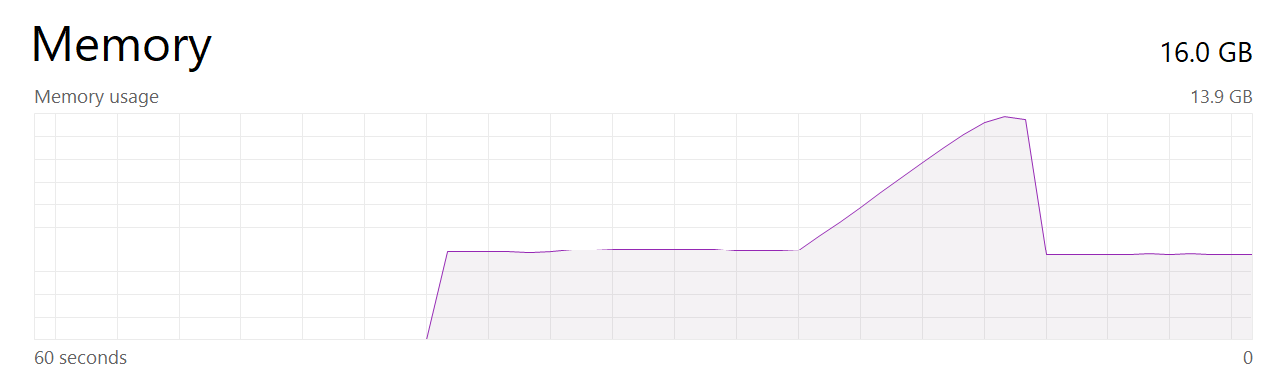
\includegraphics[width=0.8\textwidth]{../images/generalized_parts/05_memory_leak_and_after_end_task.png}
    \caption{开始运行内存泄漏器和结束运行时,内存占用的变化}
\end{figure}
图中可以看到,在我们开始运行这个程序的那一刻,内存占用就迅速增加,直到接近最大值。而在我们结束这个程序的时候,内存占用马上又回到了原来的水平。所以对于个人电脑来说,内存泄漏是无关紧要的小问题,结束一下进程,它就解决了。\par
但是不是任何时候都可以靠结束进程来解决问题的。对于需长期运行的服务器来说,贸然结束进程可以意味着很大的损失。所以在我们日常写代码的时候就要养成良好的习惯,不要写出会导致内存泄漏的代码来。\par
那么怎么预防内存泄漏呢?唯一的方法就是及时回收(或者叫释放)那些我们不需要的内存空间。\par
回收内存空间需要用到 \lstinline@delete@ 或 \lstinline@delete[]@ 运算符。其中  \lstinline@delete@ 运算符用于回收 \lstinline@new@ 分配的内存空间,而 \lstinline@delete[]@ 运算符用于回收 \lstinline@new[]@ 分配的内存空间。它们两个是不同的,一定不要混用!\par
\begin{lstlisting}
    int *pobj = new int;
    delete pobj; //使用new分配的动态内存要用delete回收
    pobj = nullptr;
    double *arr = new double[4];
    delete[] arr; //使用new[]分配的动态数组要用delete[]回收,[]内无需加数字
    arr = nullptr;
\end{lstlisting}
读者需要注意的是,\lstinline@delete@/\lstinline@delete[]@ 只是回收了这个指针所指向的动态内存,它不会影响 指针的值。那么在动态内存回收之后,这个指针指向的就是无效区域——换句话说,它是野指针!那么为了防范野指针的出现,我们最好在回收内存空间之后,让这个指针指向 \lstinline@nullptr@(\lstinline@nullptr@ 是对所有指针都绝对安全的避风港)。\par
真实情况下的内存泄漏往往往不是由这么低级的``忘记回收''导致的,而是一些``我们自己都没想到需要回收''的情况,比如
\begin{lstlisting}
int* alloc(int value) { //注意返回类型是int*,它意味着返回一个地址值
    return new int {value}; //直接返回由new分配好的动态空间,已经用value初始化
}
int main() {
    const int N {10};
    int *p[N]{}; //定义由N个指针构成的指针数组
    p[0] = alloc(5); //让将p[0]指向alloc分配好的动态内存空间
    //在经历了很多操作之后
    delete p[0]; //最后记得回收!
    return 0;
}
\end{lstlisting}
我们很容易在复杂的代码中忘记了回收动态内存空间,尤其是在这种``\lstinline@new@ 出现在一个函数中,而使用这个动态内存却是在另一个函数中''的情形下(类似的例子,我们会在面向对象编程时见得很多)。所以动态内存分配的灵活性与危险性是并存的,我们稍有不慎,就可能会造成内存泄漏的问题。\par
\subsection*{二维数组的动态内存分配}
现在你已经学会了如何动态分配一个一维数组,那么如何动态分配一个二维数组呢?我们想,二维数组也只不过是一个``一维数组类型的一维数组'',所以我们用一维数组的动态内存分配语法就足以分配一个二维数组了。
\begin{lstlisting}
    int n;
    cin >> n;
    int (*pta)[10] = new int[n][10];
\end{lstlisting}
在这里,\lstinline@new[]@ 的返回值是一个 \lstinline@(int*)[10]@,也就是指向数组的指针,我们可以定义一个 \lstinline@pta@ 来存储这个返回值。这样,我们就用一个指向 \lstinline@10@ 长度 \lstinline@int@ 数组的指针,指向了一个 \lstinline@n@ 长度的 \lstinline@10@ 长度 \lstinline@int@ 动态数组。这话可能有点绕,读者多琢磨一下想必就可以理解。\par
回收这个数组的方式很简单,直接 \lstinline@delete[]@ 就行。
\begin{lstlisting}
    delete[] pta; //回收pta指向的动态内存
    pta = nullptr; //最好这样
\end{lstlisting}\par
但是这样也有一个限制——我们在这里定义的是一个 \lstinline@n*10@ 大小的数组,还是有一个维度需要静态分配的。我们能不能让两个维度都是变量,比如定义一个 \lstinline@n*m@ 动态数组?其实是可以的。\par
我们的思路是,先用一个二阶指针,分配一个动态指针数组:
\begin{lstlisting}
    int **pp = new int*[n] {}; //全部初始化为nullptr
\end{lstlisting}
在这里,\lstinline@new@ 的返回值是一个 \lstinline@int*[n]@,也就是长度为 \lstinline@n@ 的指针数组。那么其中随便一个 \lstinline@pp[i]@ 都是一个 \lstinline@int*@ 指针,工我们岂不是可以直接为每个这样的指针分配一个长度为 \lstinline@m@ 的动态数组?
\begin{lstlisting}
    for(int i=0; i<n; i++) { //别忘了pp下标的范围是0~n-1,而不是1~n
        pp[i] = new int[m] {}; //对其中的每个指针pp[i]都分配一个长度为m的数组
    }
\end{lstlisting}
至于这种二维数组的回收,那就有讲究了。我们首先为 \lstinline@pp@ 分配了一个 \lstinline@int*@ 指针数组,然后又为其中的每个 \lstinline@int*@ 指针分配了一个 \lstinline@int@ 数组,所以这些内容都要回收(仅回收 \lstinline@pp@ 指向的空间不代表回收了每个\lstinline@pp[i]@ 指向的空间)。但是怎么回收就是个问题了——
\begin{lstlisting}
    delete[] pp; //回收pp指向的空间
    for(int i=0; i<n; i++) {
        delete[] pp[i]; //错误!
    }
\end{lstlisting}
我们仔细想一遍过程就知道为什么了:当 \lstinline@pp@ 的空间被回收之后,\lstinline@pp@ 就变成了一个野指针。这时候再访问它的内容就不合理了,所以 \lstinline@pp[i]@ 这个用法也就有问题了!\par
所以我们回收动态内存的时候也要讲求一个顺序。应该先回收各个 \lstinline@pp[i]@ 的空间,然后再回收 \lstinline@pp@ 的空间才对。\par
\begin{lstlisting}
    for(int i=0; i<n; i++) {
        delete[] pp[i]; //先回收各个pp[i]的空间
    }
    delete[] pp; //再回收pp的空间
\end{lstlisting}\par
